% Universidade Aberta
% Template TeX para relatório de trabalhos
% 2025
%
%
% Dados para a capa
\newcommand{\Titulo}{Planeamento e Desenvolvimento de Sistemas de Informação}
\newcommand{\SubTitulo}{Trabalho Grupo - Topico 3}
\newcommand{\Ano}{2025}
\newcommand{\Autor}{
    Pedro Morais - 2401849 \\
    Hugo Gonçalves - 2100562 \\
    Pedro Moro - 2001642 \\
    Luis Peixoto - 2402741 \\
}
%
%
\documentclass[12pt,a4paper,final]{article}
\usepackage{csquotes}
\usepackage{float}
\usepackage[portuguese]{babel}
\usepackage{polyglossia}
\setdefaultlanguage{portuguese}
\usepackage{graphicx}
\graphicspath{ {./images/} }
\usepackage[a4paper,top=3cm,bottom=3cm,left=3.5cm,right=2cm]{geometry}
\usepackage{booktabs}
\setmainfont{Times New Roman}
\defaultfontfeatures{Ligatures=TeX}
\usepackage[pdfauthor=\Autor,
    pdftitle=\Titulo,
    colorlinks=true,
    linkcolor=black,
    citecolor=black,
    bookmarksopen=true]{hyperref}
\hypersetup{colorlinks, citecolor=black, urlcolor=black}
\usepackage{bookmark}
\usepackage[style=apa, backend=biber, sortcites, url=true, language=portuguese]{biblatex}
\usepackage{fontspec}
\DeclareLanguageMapping{portuguese}{portuguese-apa}
\addbibresource{ref.bib}
\renewcommand{\baselinestretch}{1.5}
\begin{document}
    \title{\Titulo}
    \author{\Autor}
    \date{\Ano}
    \pagenumbering{gobble}
    \begin{titlepage}
        \begin{center}
            \vspace*{4cm}

            \textbf{\large UNIVERSIDADE ABERTA}

            \textbf{\large UNIVERSIDADE DE TRÁS-OS-MONTES E ALTO DOURO}

            \vspace{1cm}

            \begin{minipage}{0.4\textwidth}
                \centering
                
\includegraphics[width=0.8\textwidth]{uab}
            \end{minipage}
            \begin{minipage}{0.4\textwidth}
                \centering
                
\includegraphics[width=0.8\textwidth]{utad}
            \end{minipage}

            \vspace{1.5cm}

            \textbf{\large \Titulo}

            \textbf{\large \SubTitulo}

            \vspace{1.5cm}

            \textbf{\large \Autor}

            \vspace{2cm}

            \textbf{\large Mestrado em Engenharia Informática e Tecnologia Web}
            \vfill
            \textbf{\Ano}
        \end{center}
    \end{titlepage}
    \renewcommand{\contentsname}{Índice}
    \cleardoublepage
    \pagenumbering{roman}
    \tableofcontents
    \newpage
    \listoffigures
    \newpage
    \cleardoublepage
    \pagenumbering{arabic}

    \section*{Introdução}\label{sec:introducao}
    \addcontentsline{toc}{section}{Introdução}
    O presente relatório tem como objetivo a caracterização da arquitectura empresarial da Direção Municipal de Higiene Urbana (DMHU), unidade funcional da Câmara Municipal de Lisboa (CML), no seu estado atual (`AS-IS').
    Este trabalho insere-se no âmbito da unidade curricular de Planeamento e Desenvolvimento de Sistemas de Informação (PDSI), e serve de base para uma futura transformação da organização.

    Este trabalho constitui uma etapa fundamental para a futura definição do modelo `TO-BE`, essencial para a transição de Lisboa para uma cidade inteligente (`Smart City`).

    A caracterização `AS-IS` permite identificar a estrutura organizacional existente, os principais atores envolvidos, internos e externos, os processos de negócio e as aplicações informáticas que suportam as atividades da DMHU. O objetivo é obter uma visão clara do funcionamento atual da organização, dos fluxos de informação e das interações com os stakeholders, de forma a fundamentar decisões estratégicas e propostas de melhoria.

    Neste relatório, são abordadas várias dimensões da arquitetura empresarial, organizadas segundo os pontos de vista definidos pela linguagem ArchiMate.
    A modelação foi realizada com recurso a diagramas que acompanham o presente documento, incluindo:

    \begin{itemize}
        \item \textbf{Contexto Organizacional e Atores Envolvidos};
        \item \textbf{Produtos e Serviços Prestados};
        \item \textbf{Estrutura Organizacional da DMHU};
        \item \textbf{Processos e Relação com os Serviços};
        \item \textbf{Especificação dos Processos de Negócio};
    \end{itemize}

    Para além das figuras representativas dos modelos ArchiMate, este relatório inclui descrições detalhadas dos elementos envolvidos, servindo não apenas como instrumento de comunicação visual, mas também como documento interpretativo da arquitetura organizacional e dos fluxos operacionais.

    Este trabalho baseia-se em documentos oficiais e académicos, nomeadamente o relatório de atividades da DMHU, documentos de estrutura organizacional, documentação sobre os processos internos e externos da organização, bem como referências do Open Group e do modelo APQC. Através desta análise integrada, procura-se criar uma base sólida para o planeamento futuro da arquitetura empresarial da CML, com foco na eficiência, sustentabilidade e digitalização dos processos de negócio.


    \section*{Q1 - Contexto Organizacional e Atores Envolvidos}\label{sec:contexto-organizacional-e-atores-envolvidos}
    \addcontentsline{toc}{section}{Q1 - Contexto Organizacional e Atores Envolvidos}
    A DMHU integra-se na estrutura funcional da Câmara Municipal de Lisboa, sendo responsável pela gestão de resíduos e higiene urbana.
    \begin{itemize}
        \item Cidadãos de Lisboa (reclamações, ocorrências, pedidos);
        \item Juntas de Freguesia (intervenções locais, eventos);
        \item Entidades Reguladoras (ex: ERSAR);
        \item Polícia Municipal (fiscalização);
        \item Fornecedores e prestadores de serviços.
    \end{itemize}

    \begin{figure}[H]
        \centering
        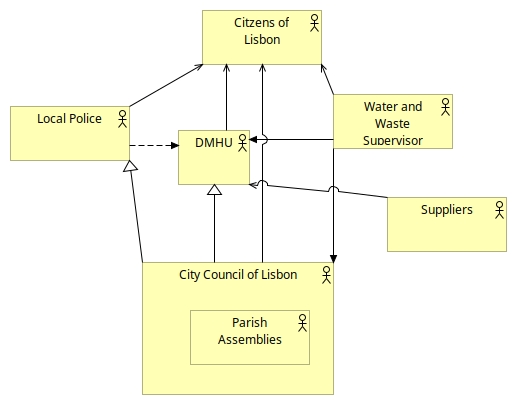
\includegraphics[width=0.45\textwidth]{Q1 - DHMU Context}
        \caption{Modelo ArchiMate — Cooperação com Atores Externos}
        \label{fig:1}
    \end{figure}

    \section*{Q2 - Produtos e Serviços Prestados}\label{sec:produtos-e-servicos-prestados}
    \addcontentsline{toc}{section}{Q2 - Produtos e Serviços Prestados}
    A DMHU presta os seguintes serviços à cidade:
    \begin{itemize}
        \item Higiene Urbana;
        \item Limpeza Urbana;
        \item Projetos de Higiene;
        \item Transporte;
        \item Sensibilização Ambiental;
        \item Gestão de Garagens e Oficinas.
    \end{itemize}

    \begin{figure}[H]
        \centering
        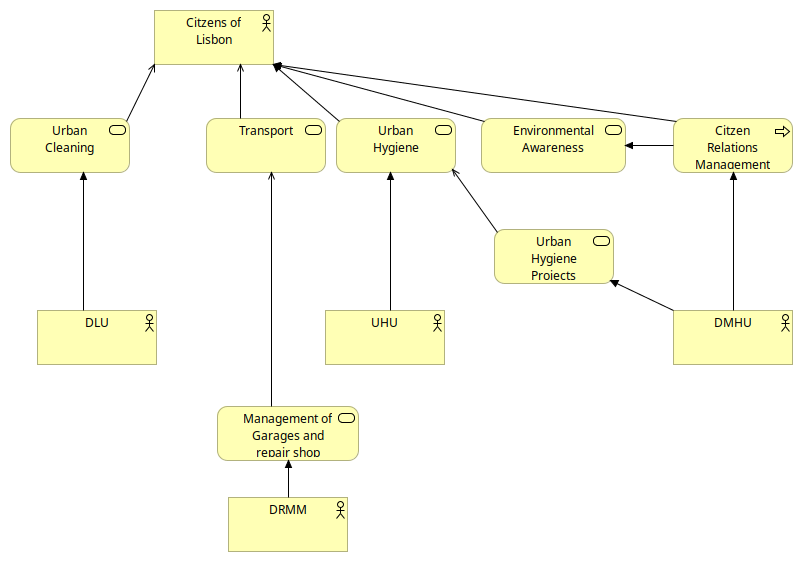
\includegraphics[width=0.6\textwidth]{Q2 - Business Services}
        \caption{Serviços Prestados pela DMHU}
        \label{fig:2}
    \end{figure}

    Estes serviços respondem às necessidades operacionais do município e estão alinhados com os objetivos estratégicos definidos no Relatório de Atividades de 2015.

    \section*{Q3 - Estrutura Organizacional da DMHU}\label{sec:estrutura-organizacional-da-dmhu}
    \addcontentsline{toc}{section}{Q3 - Estrutura Organizacional da DMHU}
    A estrutura da DMHU está dividida em dois departamentos principais:
    \begin{itemize}
        \item \textbf{DHU} – Departamento de Higiene Urbana (inclui DLU e UHU);
        \item \textbf{DRMM} – Departamento de Reparação e Manutenção Mecânica (inclui DGF e DMF).
    \end{itemize}

    \begin{figure}[H]
        \centering
        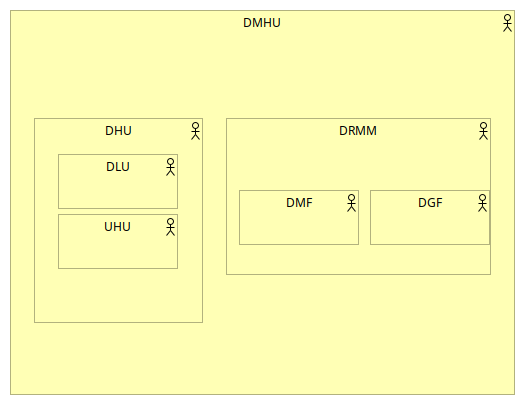
\includegraphics[width=0.85\textwidth]{Q3 - Organizational Structure}
        \caption{Organograma DMHU — Modelo ArchiMate}
        \label{fig:3}
    \end{figure}

    \begin{figure}[H]
        \centering
        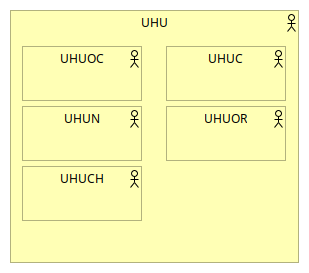
\includegraphics[width=0.65\textwidth]{Q3 - Organizational Structure - UHU}
        \caption{Organograma DMHU UHU — Modelo ArchiMate}
        \label{fig:10}
    \end{figure}

    \newpage

    \section*{Q4 - Processos e Relação com os Serviços}\label{sec:processos-e-relacao-com-os-servicos}
    \addcontentsline{toc}{section}{Q4 - Processos e Relação com os Serviços}
    Os serviços identificados anteriormente são suportados por cinco macroprocessos:
    \begin{itemize}
        \item Gestão da Recolha de Resíduos;
        \item Relação com o Cidadão;
        \item Gestão de Recursos Humanos;
        \item Gestão do Armazém;
        \item Gestão da Frota.
    \end{itemize}

    \begin{figure}[H]
        \centering
        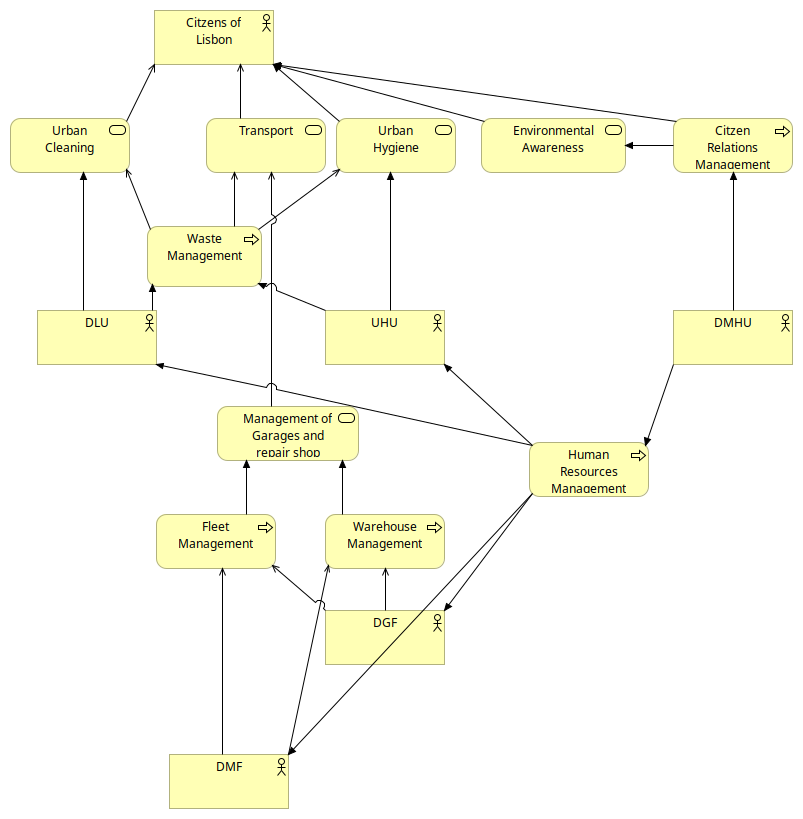
\includegraphics[width=0.65\textwidth]{Q4 - Relation Between Business services and Business Processes}
        \caption{Relação entre Serviços e Processos}
        \label{fig:4}
    \end{figure}

    \section*{Q5 - Especificação dos Processos de Negócio}\label{sec:especificacao-dos-processos-de-negocio}
    \addcontentsline{toc}{section}{Q5 - Especificação dos Processos de Negócio}
    Cada macroprocesso inclui subprocessos detalhados:
    \begin{itemize}
        \item Recolha de Resíduos: Planeamento, Execução, Registo;
        \item Relação com o Cidadão: Interação com GOPI, Avaliação de Pedidos;
        \item Recursos Humanos: Registos, Formação, Férias, Fardamento;
        \item Frota: Manutenção, Alocação de Viaturas;
        \item Armazém: Gestão de Stocks, Requisições, Armazenamento.
    \end{itemize}

    \begin{figure}[H]
        \centering
        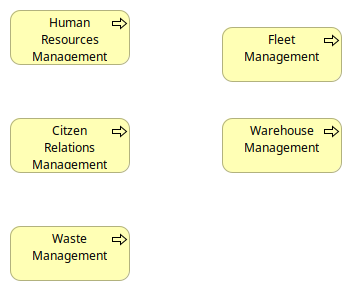
\includegraphics[width=0.6\textwidth]{Q5 - High Level Specification of Business Process}
        \caption{Modelo de Processos de Negócio — ArchiMate}
        \label{fig:5}
    \end{figure}

    \section*{Q7 - Sumário das Entidades de Informação da DMHU}
    \addcontentsline{toc}{section}{Q7 - Sumário das Entidades de Informação DMHU}
    A Tabela~\ref{tab:inmon} sintetiza as principais entidades identificadas nas
    camadas Transacional e de \textit{Business Intelligence} (BI), atribuindo-lhes a
    classificação proposta por Inmon para um armazém de dados—\emph{current
    detail}, \emph{lightly summarized} ou \emph{historical detail}—consoante a sua
    granularidade e horizonte temporal.

    \begin{table}[]
        \centering
        \caption{Classificação Inmon das entidades de informação da DMHU}
        \label{tab:inmon}
        \begin{tabular}{@{}|c|c|c|@{}}
            \toprule
            \textbf{Entidade} & \textbf{Identificador (PK)} & \textbf{Classificacao Inmon}\\\midrule
            Equipamentos\_Execucao          & \texttt{ExecucaoID}         & Current detail\\
            Cadastro\_Circuitos             & \texttt{CircuitoID}         & Current detail\\
            Execucao\_Diária                & \texttt{ExecucaoID}         & Current detail\\
            Escala\_Circuitos               & \texttt{EscalaID}           & Current detail\\
            Cadastro\_PRS                   & \texttt{PRSID}             & Current detail\\
            Equipamentos                    & \texttt{EquipamentoID}      & Current detail\\
            Solicitacoes\_Ocorrencias       & \texttt{OcorrenciaID}       & Current detail\\
            Pessoas\_Escala\_Circuitos      & \texttt{PessoaEscalaID}     & Current detail\\
            RH\_Fardamento\_EPI             & \texttt{EPIID}              & Current detail\\
            Manutencao                      & \texttt{ManutencaoID}       & Current detail\\
            Interacoes                      & \texttt{InteracaoID}        & Current detail\\
            Cadastro\_Colaboradores         & \texttt{ColaboradorID}      & Historical detail\\
            Acidentes\_Colaboradores        & \texttt{AcidenteID}         & Historical detail\\
            RH\_SIADAP                       & \texttt{AvaliacaoID}        & Historical detail\\
            RH\_Ocorrencias                 & \texttt{RH\_OcorrenciaID}   & Historical detail\\
            RH\_Formacao\_Colaborador       & \texttt{FormacaoColabID}    & Historical detail\\
            RH\_Acidentes                   & \texttt{AcidenteID}          & Historical detail\\
            RH\_Formacao                   & \texttt{FormacaoID}        & Historical detail\\
            Orcamento                       & \texttt{OrcamentoID}    & Historical detail\\
            \midrule
            \multicolumn{3}{p{12cm}}{\textit{Nota:} as réplicas diárias destas entidades na
            camada BI são classificadas como \emph{lightly summarized}, correspondendo a
            snapshots temporais para análise e \textit{report}.}\\
            \bottomrule
        \end{tabular}
    \end{table}
    \newpage
    \section*{Q8 - Modelo de Domínio Detalhado}
    \addcontentsline{toc}{section}{Q8 - Modelo de Domínio Detalhado}

    \subsection*{Class Diagram UML}\label{subsec:class-diagram-uml}
    A Figura~\ref{fig:uml-detalhado} apresenta o diagrama de classes
    detalhado, já partilhado anteriormente, que cobre os relacionamentos de todas
    as entidades transacionais.

    \begin{figure}[H]
        \centering
        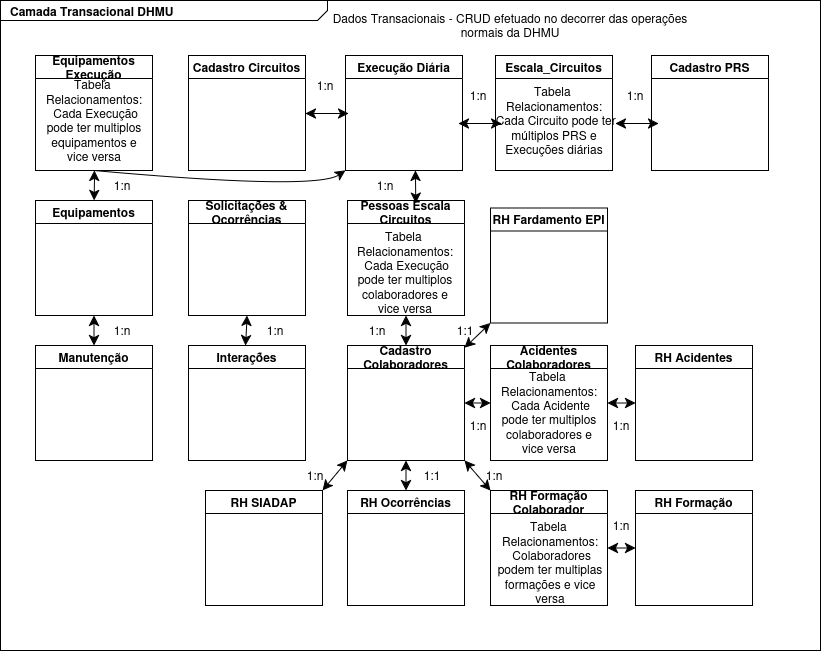
\includegraphics[width=\textwidth]{UML}
        \caption{Diagrama de classes UML das entidades transacionais da DMHU.}
        \label{fig:uml-detalhado}
    \end{figure}

    \subsection*{Information Structure \textit{ArchiMate}}\label{subsec:information-structure-archimate}
    Complementarmente, a Figura~\ref{fig:archi-info} utiliza o
    \textit{viewpoint} \emph{Information Structure} de ArchiMate para evidenciar
    como os objetos de dados são replicados e disponibilizados na camada BI,
    estabelecendo a ponte entre dados operacionais e informacionais.

    \begin{figure}[H]
        \centering
        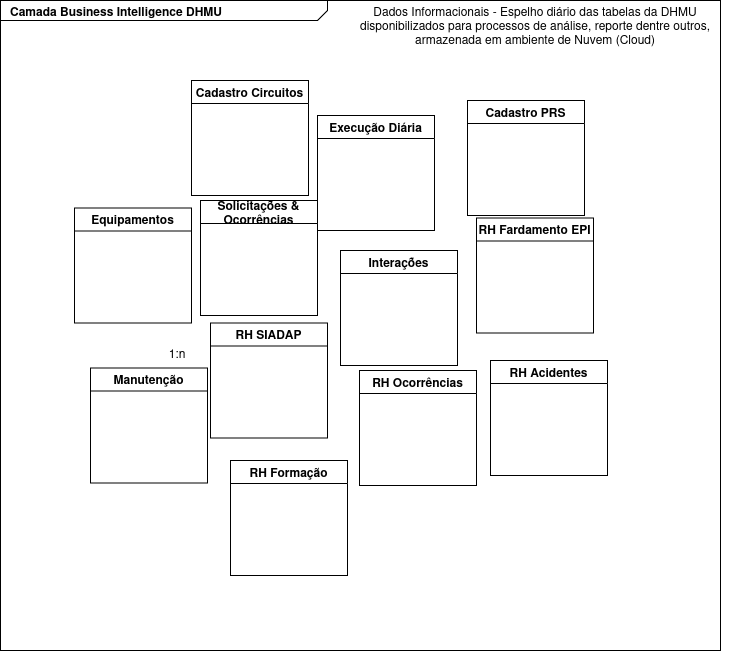
\includegraphics[width=\textwidth]{CAMADA}
        \caption{Vista \textit{Information Structure} (ArchiMate) – espelho diário das
        entidades para BI.}
        \label{fig:archi-info}
    \end{figure}

    Estas duas representações asseguram uma visão consistente
    (\emph{traceability}) entre o modelo de domínio e a arquitetura de dados,
    facilitando a evolução futura da solução.

    \newpage
    \nocite{*}
    \printbibliography
\end{document}